\documentclass[a4paper, 13pt]{article}
\usepackage[utf8]{inputenc}
\usepackage{graphicx}
\usepackage{multirow}
\usepackage{geometry}
\usepackage[french]{babel}
\geometry{
margin=1cm,
bottom=0.25cm,
top=3.4cm,
paperwidth=34.18cm,
paperheight=21cm
}
\usepackage{hyperref}
\usepackage{fix-cm}
\usepackage{enumitem}
\usepackage{qrcode}
\graphicspath{ {\VAR{image_path}} }
\pagestyle{empty}
\author{IFNTI}
\title{carte_etudiant}
\usepackage{eso-pic}

\makeatletter
\newcommand\HUGE{\@setfontsize\Huge {30}{36}}
\newcommand\Larged{\@setfontsize\Larged {20.4}{18}}
\makeatother

\newcommand\BackgroundPicCorps{
\put(0,0){
\parbox[b][\paperheight]{\paperwidth}{
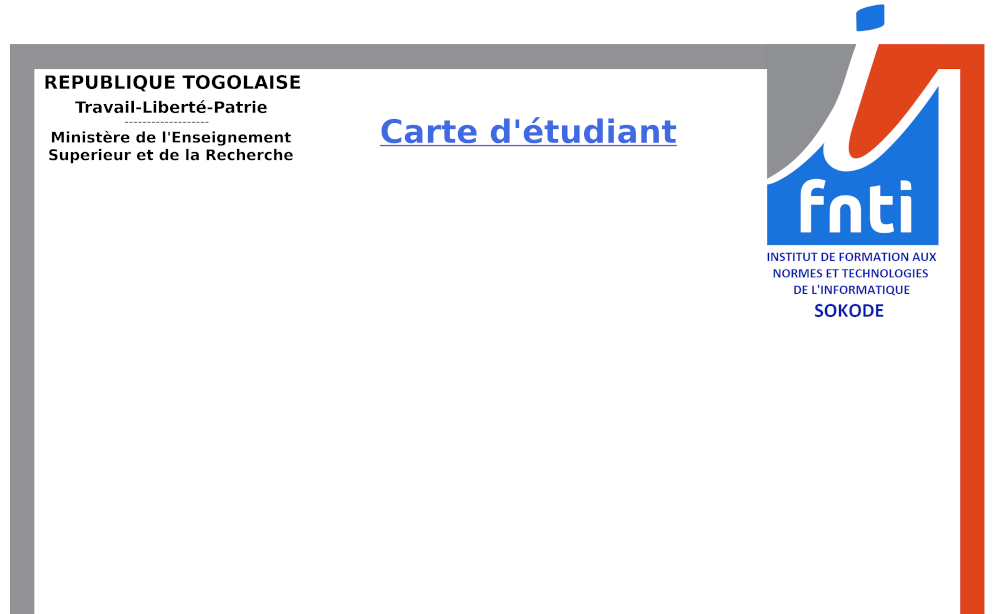
\includegraphics[width=\paperwidth,height=\paperheight]{carte_graphique6.png}
}}}

\newcommand\BackgroundPicVerso{
\put(0,0){
\parbox[b][\paperheight]{\paperwidth}{

\includegraphics[width=\paperwidth,height=\paperheight]{carte_graphique_verso2.png}
}}}

\begin{document}
\AddToShipoutPicture{\BackgroundPicCorps}
\noindent
\BLOCK{ for etudiant in etudiants }
\vspace*{2.5cm}

\HUGE
%\vfill

%\begin{table}
%\resizebox{0.75\textwidth}{!}{

\begin{tabular}{lll}
\multirow {8}{7cm}{\includegraphics[width=7cm]{\VAR{etudiant.photo}}}
   		& Matricule : & \VAR{ etudiant.id } \\ 
  		& Nom : & \VAR{ etudiant.nom } \\ 
 		& Prénom :  & \VAR{ etudiant.prenom }\\ 
 		& Né le : & \VAR{ etudiant.datenaissance }\\ 
 		& A: & \VAR{ etudiant.lieunaissance } \\ 
 		& Sexe : & \VAR{ etudiant.sexe } \\ 
 		& Adresse : & \VAR{ etudiant.adresse }\\ 
 		& Tél : & \VAR{ etudiant.contact}\\ 

\end{tabular} %}
%\end{table}

\vspace{-1cm}
\huge
\begin{minipage}{0.35\textwidth}
\vspace{2cm}
\begin{center}
Licence LMD\\
\vspace{0.5cm}
Informatique des organisations\\
\end{center}
\end{minipage}
\hfill
\begin{minipage}{0.3\textwidth}
\begin{center}
\vspace{0cm}
Sokodé, le \today\\
\vspace{0cm}
Le Directeur\\
\vspace{0cm}


\vspace{3cm}
Sabirou TEOURI\\
\end{center}
\end{minipage}

\newpage

\AddToShipoutPictureBG*{\BackgroundPicVerso}

\newgeometry{left=1.5cm, bottom=1cm, top=3.4cm,}

\HUGE

\noindent
\begin{minipage}{0.6\textwidth}
\vspace{2cm}
IFNTI Sokodé\\
300 BP 40\\
Tél: 90 91 31 41\\
Site web: https://www.ifnti.com\\
\end{minipage}
\hfill
\begin{minipage}{0.2\textwidth}
\vspace{-2cm}
\qrcode[height=3in]{\VAR{ etudiant.qrcode }}\\
\end{minipage}

%\vfill

\noindent
Année Academique {\color{blue} \VAR{annee}} \hspace{1cm} Niveau {\color{blue} \VAR{etudiant.niveau}}\\

\vspace{-0.25cm}
%\vfill

%\noindent
%Personne à prévenir
%\begin{description}
%\item[$\ast$] \VAR{etudiant.personnePrevenir}
%\item[$\ast$] Tél:  \VAR{etudiant.contact}
%\end{description}

\noindent
\begin{tabular}{ccc}
Personne à prévenir : & \VAR{etudiant.tuteurs.nom} & (\VAR{etudiant.tuteurs.contact})
\end{tabular}

\vspace{1cm}

%\begin{minipage}{0.27\textwidth}
%Personne à prévenir : 
%\end{minipage}
%\hfill
%\begin{minipage}{0.47\textwidth}
%\VAR{etudiant.personnePrevenir}
%\end{minipage}
%\hfill
%\begin{minipage}{0.2\textwidth}
%Tél :  \VAR{etudiant.contact}
%\end{minipage}

%\vfill

\noindent
Observations importantes\\
- Cette carte est stritement personnelle \\
- Toute fraude constatée donnera lieu à des poursuites
%- La validité de cette carte couvre tout le parcours académique

\newpage

\BLOCK{endfor}

%\vspace{2cm}

\end{document}